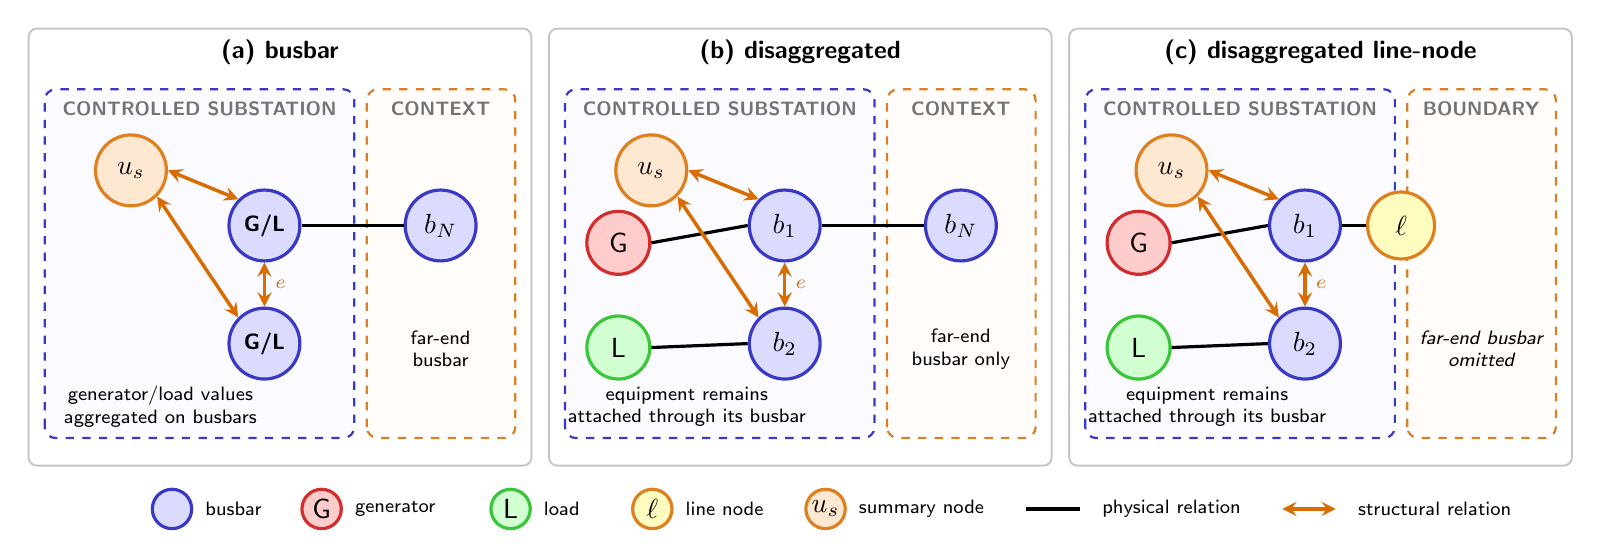
\begin{tikzpicture}[
  x=1cm,
  y=1cm,
  >=stealth,
  font=\sffamily,
  busbar/.style={
    circle,
    draw=blue!55!gray,
    fill=blue!14,
    line width=1.15pt,
    minimum size=9mm,
    inner sep=0pt
  },
  generator/.style={
    circle,
    draw=red!65!gray,
    fill=red!20,
    line width=1.15pt,
    minimum size=8mm,
    inner sep=0pt
  },
  load/.style={
    circle,
    draw=green!55!gray,
    fill=green!18,
    line width=1.15pt,
    minimum size=8mm,
    inner sep=0pt
  },
  linenode/.style={
    circle,
    draw=orange!75!gray,
    fill=yellow!25,
    line width=1.15pt,
    minimum size=8.5mm,
    inner sep=0pt
  },
  summary/.style={
    circle,
    draw=orange!75!gray,
    fill=orange!18,
    line width=1.15pt,
    minimum size=9mm,
    inner sep=0pt
  },
  physical/.style={draw=black, line width=1.15pt},
  structural/.style={<->, draw=orange!85!black, line width=1.25pt},
  panel/.style={draw=gray!45, rounded corners=3pt, line width=0.7pt},
  controlled/.style={
    draw=blue!55!gray,
    dashed,
    rounded corners=4pt,
    fill=blue!2,
    line width=0.8pt
  },
  context/.style={
    draw=orange!70!gray,
    dashed,
    rounded corners=4pt,
    fill=orange!2,
    line width=0.8pt
  },
  zone/.style={font=\scriptsize\bfseries\sffamily, text=gray!75},
  title/.style={font=\small\bfseries\sffamily},
  note/.style={font=\scriptsize\sffamily, align=center},
  omitted/.style={font=\scriptsize\itshape\sffamily, align=center, text=gray!68}
]

% Both augmentations are enabled in every panel.  Their placement is invariant:
% e joins controlled busbars and n joins the controlled busbars to u_s.

% ---------------------------------------------------------------------------
% (a) Busbar representation
% ---------------------------------------------------------------------------
\begin{scope}[xshift=-39pt, xscale=1.13]
  \path[panel] (0,0) rectangle (5.65,5.55);
  \node[title] at (2.825,5.25) {(a) busbar};
  \path[controlled] (0.18,0.35) rectangle (3.66,4.78);
  \path[context] (3.80,0.35) rectangle (5.47,4.78);
  \node[zone, text=black!55] at (1.92,4.53) {CONTROLLED SUBSTATION};
  \node[zone, text=black!55] at (4.63,4.53) {CONTEXT};

  \node[summary] (bus-u) at (1.15,3.75) {$u_s$};
  \node[busbar, node font=\footnotesize\sffamily\bfseries] (bus-b1) at (2.65,3.05) {G/L};
  \node[busbar, node font=\footnotesize\sffamily\bfseries] (bus-b2) at (2.65,1.55) {G/L};
  \node[busbar] (bus-bn) at (4.63,3.05) {$b_N$};

  \draw[physical] (bus-b1.east) -- (bus-bn.west);
  \draw[structural] (bus-b1.south) --
    node[note, right, text=orange!85!black] {$e$} (bus-b2.north);
  \draw[structural] (bus-u.east) -- (bus-b1.north west);
  \draw[structural] (bus-u.south east) -- (bus-b2.north west);

  \node[note] at (1.48,0.75) {generator/load values\\aggregated on busbars};
  \node[note] at (4.63,1.48) {far-end\\busbar};
\end{scope}

% ---------------------------------------------------------------------------
% (b) Disaggregated representation
% ---------------------------------------------------------------------------
\begin{scope}[xshift=149pt, xscale=1.13]
  \path[panel] (0,0) rectangle (5.65,5.55);
  \node[title] at (2.825,5.25) {(b) disaggregated};
  \path[controlled] (0.18,0.35) rectangle (3.66,4.78);
  \path[context] (3.80,0.35) rectangle (5.47,4.78);
  \node[zone, text=black!55] at (1.92,4.53) {CONTROLLED SUBSTATION};
  \node[zone, text=black!55] at (4.63,4.53) {CONTEXT};

  \node[summary] (het-u) at (1.15,3.75) {$u_s$};
  \node[generator] (het-g) at (0.78,2.83) {G};
  \node[load] (het-l) at (0.78,1.50) {L};
  \node[busbar] (het-b1) at (2.65,3.05) {$b_1$};
  \node[busbar] (het-b2) at (2.65,1.55) {$b_2$};
  \node[busbar] (het-bn) at (4.63,3.05) {$b_N$};

  \draw[physical] (het-g.east) -- (het-b1.west);
  \draw[physical] (het-l.east) -- (het-b2.west);
  \draw[physical] (het-b1.east) -- (het-bn.west);
  \draw[structural] (het-b1.south) --
    node[note, right, text=orange!85!black] {$e$} (het-b2.north);
  \draw[structural] (het-u.east) -- (het-b1.north west);
  \draw[structural] (het-u.south east) -- (het-b2.north west);

  \node[note] at (1.55,0.75) {equipment remains\\attached through its busbar};
  \node[note] at (4.63,1.48) {far-end\\busbar only};
\end{scope}

% ---------------------------------------------------------------------------
% (c) Disaggregated representation with explicit line nodes
% ---------------------------------------------------------------------------
\begin{scope}[xshift=337pt, xscale=1.13]
  \path[panel] (0,0) rectangle (5.65,5.55);
  \node[title] at (2.825,5.25) {(c) disaggregated line-node};
  \path[controlled] (0.18,0.35) rectangle (3.66,4.78);
  \path[context] (3.80,0.35) rectangle (5.47,4.78);
  \node[zone, text=black!55] at (1.92,4.53) {CONTROLLED SUBSTATION};
  \node[zone, minimum width=52pt, text=black!55] at (4.63,4.53) {BOUNDARY};

  \node[summary] (line-u) at (1.15,3.75) {$u_s$};
  \node[generator] (line-g) at (0.78,2.83) {G};
  \node[load] (line-l) at (0.78,1.50) {L};
  \node[busbar] (line-b1) at (2.65,3.05) {$b_1$};
  \node[busbar] (line-b2) at (2.65,1.55) {$b_2$};
  \node[linenode] (line-ln) at (3.73,3.05) {$\ell$};

  \draw[physical] (line-g.east) -- (line-b1.west);
  \draw[physical] (line-l.east) -- (line-b2.west);
  \draw[physical] (line-b1.east) -- (line-ln.west);
  \draw[structural] (line-b1.south) --
    node[note, right, text=orange!85!black] {$e$} (line-b2.north);
  \draw[structural] (line-u.east) -- (line-b1.north west);
  \draw[structural] (line-u.south east) -- (line-b2.north west);

  \node[note] at (1.55,0.75) {equipment remains\\attached through its busbar};
  \node[omitted, text=black] at (4.63,1.48) {far-end busbar\\omitted};
\end{scope}

% Compact shared legend.
\node[busbar, minimum size=5mm] at (0.45,-0.55) {};
\node[note, anchor=west] at (0.75,-0.55) {busbar};
\node[generator, minimum size=5mm] at (2.35,-0.55) {G};
\node[note, anchor=west] at (2.65,-0.55) {generator};
\node[load, minimum size=5mm] at (4.75,-0.55) {L};
\node[note, anchor=west] at (5.05,-0.55) {load};
\node[linenode, minimum size=5mm] at (6.55,-0.55) {$\ell$};
\node[note, anchor=west] at (6.85,-0.55) {line node};
\node[summary, minimum size=5mm] at (8.75,-0.55) {$u_s$};
\node[note, anchor=west] at (9.05,-0.55) {summary node};
\draw[physical] (11.30,-0.55) -- (11.98,-0.55);
\node[note, anchor=west] at (12.14,-0.55) {physical relation};
\draw[structural] (14.55,-0.55) -- (15.23,-0.55);
\node[note, anchor=west] at (15.39,-0.55) {structural relation};

\end{tikzpicture}
